\subsection*{Übertragungsmedien}

\begin{example2}{Berechnung Signaldämpfung}\\
    \includegraphics[width=0.75\linewidth]{images/example_signaldämpfung.png}
    $$U1/U2 = 1/0.5 = 2, Signaldämpfung = 20 \cdot log(2) = 6dB$$
\end{example2}

\subsubsection{Strukturierte Gebäudeverkabelung nach ISO/IEC 11801}
        \centering
        \includegraphics[width=1\linewidth]{images/Gebäudeverkabelung.png}

\subsection*{Physical Layer}

\begin{example}
    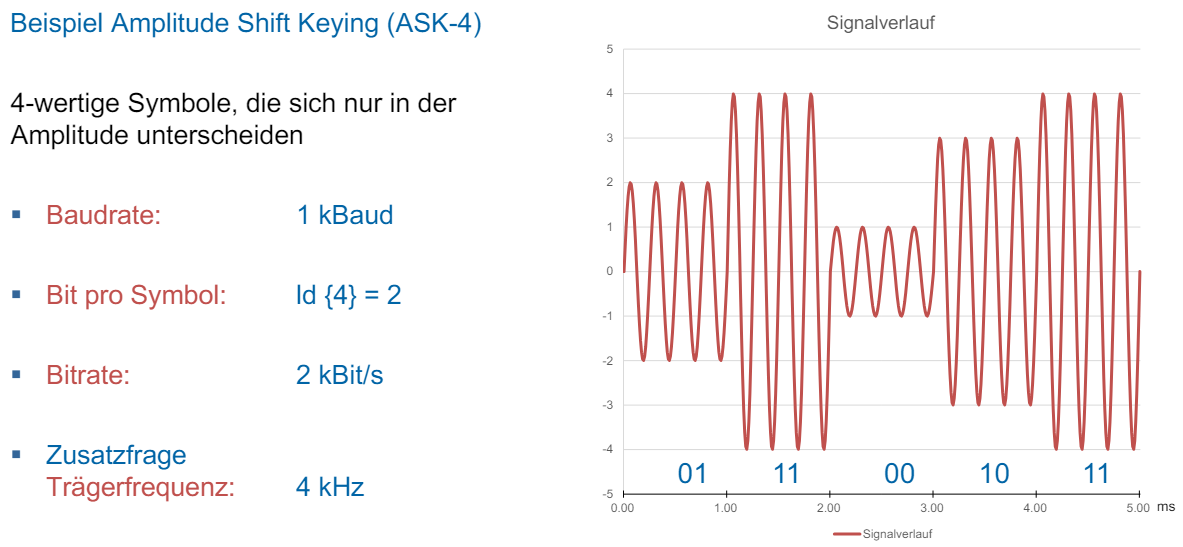
\includegraphics[width=1\linewidth]{images/amplitude_shift_keying.png}
\end{example}

\begin{concept}{AMI Leitungscode}\\
    3-wertiger AMI-Code (Alternate Mark Inversion)\\
    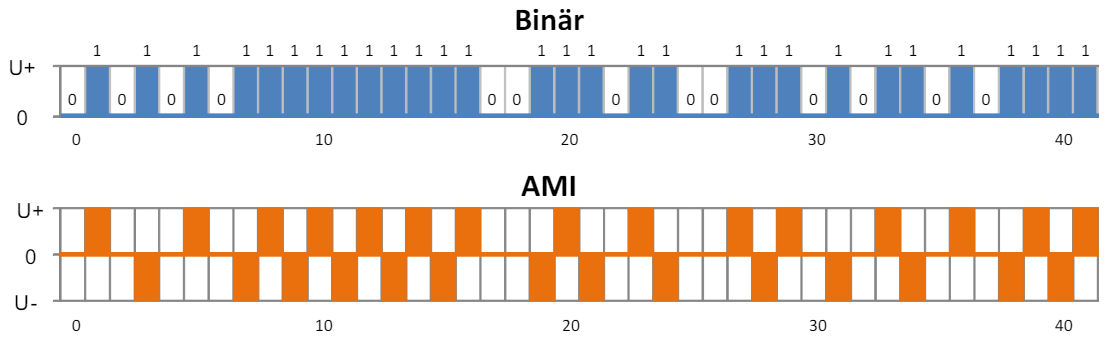
\includegraphics[width=0.8\linewidth]{images/gleichspannungsfreiheit.png}\\
    Nachteile dieses Leitungscodes:
    \begin{itemize}
        \item Auf der Übertragungsstrecke drei Zustände benötigt → rein binäre Medien genügen nicht
        \item Bei einer längeren Folge von 0 in den Daten ist keine Taktrückgewinnung mehr möglich
    \end{itemize}
\end{concept}

\begin{concept}{Manchester Leitungscode}\\
    wird z.B. bei 10BASE-T Ethernet verwendet, erlaubt einfache Taktrückgewinnung
    \begin{itemize}
        \item 1 positive Flanke, 0 negative Flanke
        \item Bei jedem Bit gibt es einen Signalwechsel
        \item Bandbreite von 10 MHz benötigt (2 $\times$ theoretisches Minimum)
    \end{itemize}
    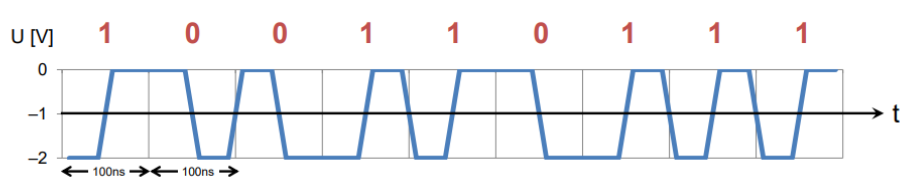
\includegraphics[width=0.6\linewidth]{images/leitungscode.png}
\end{concept}

\begin{concept}{NRZI MLT-3 Leitungscodierung}\\
    NRZI-Codierung (Non Return to Zero Inverted), kombiniert mit MLT-3\\
        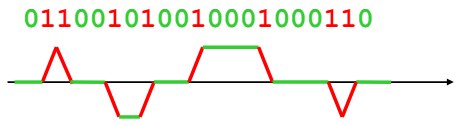
\includegraphics[width=0.5\linewidth]{images/leitungscodierung.png}\\
    MLT-3 = Multi-Level Transmit - Ternary
\end{concept}

\subsection*{Data Link Layer}

\begin{example}
    Gegeben: Bitrate 100 Mbit/s, Frame-Länge 1000 Byte, IFG 96 Bit, Payload 800 Byte. Berechnen Sie die Nutzdatenrate.\\
    \textbf{Lösung:}\\
    $$F_R = \frac{100 \cdot 10^6}{8 \cdot (1000 + 96)} = 1.19 \cdot 10^6 \text{ Frames/s}$$
    $$N = 1.19 \cdot 10^6 \cdot 800 \cdot 8 = 7.6 \cdot 10^9 \text{ Bit/s} = 7.6 \text{ Gbit/s}$$
\end{example}

\subsubsection*{LAN und Ethernet}

\begin{formula}{GBASE-T}\\
    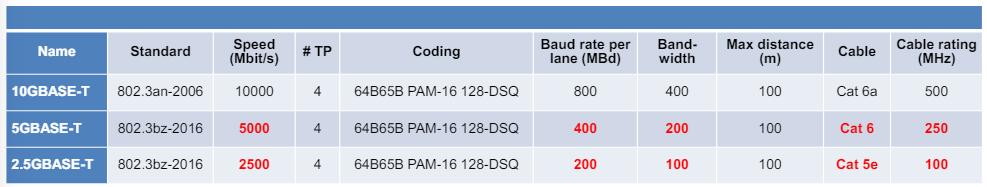
\includegraphics[width=1\linewidth]{images/GBASE-T.png}
\end{formula}

\begin{example}{100Base-TX Oszilloskop}\\
 Sie sehen auf einem Oszilloskop das folgende Bild eines 100Base-TX Signals:
  \begin{center}
  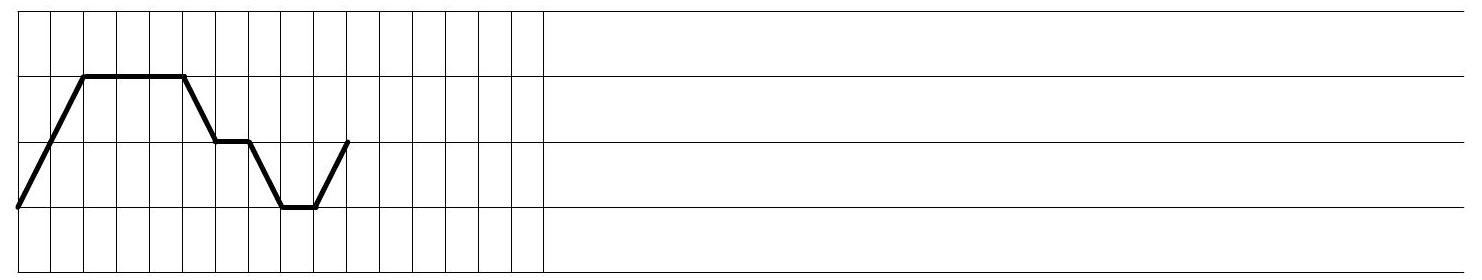
\includegraphics[width=0.8\textwidth]{images/2024-06-20-17-47-36.png}
  \end{center}
Ein Kästchen entspricht einem Bit. Wie lauten die ersten 10 Bits?

\textbf{Antwort:}\\
1100010101
\end{example}
\begin{example}{Optische übertragungsmedien}\\
    Die optische Sendeeinrichtung sendet mit $10^{-3}$ Watt Leistung. Für eine genügende Übertragungsqualität muss
    der Leistungspegel beim Empfänger mindestens $10^{-5}$ Watt betragen. Der Lichtwellenleiter hat einen
    Dämpfungsbelag von $0.5 \mathrm{~dB} / \mathrm{km}$. Welche Distanz kann überbrückt werden?

   \textbf{Antwort:}\\
Die erlaubte Abschwächung der Leistung entspricht dem Faktor 100, also $20 \mathrm{~dB}$. Demzufolge darf die Leitung maximal $40 \mathrm{~km}$ lang sein.
\end{example}
\begin{example}{maximale Bitrate}\\
 Ein Übertragungssystem nutzt eine Bandbreite von $100 \mathrm{MHz}$ und codiert den Bitstrom mit 4wertigen Symbolen.

 Welches ist die theoretisch erreichbare maximale Bitrate?

%max_Symbolrate $=200 \mathrm{MBd}$

\textbf{Antwort:}\\
%2 Bit/Symbol $\rightarrow$ max_Bitrate $=400 \mathrm{Mbit} / \mathrm{s}$
\end{example}
\begin{example}{Maximale zeichenrate}\\
Wir betrachten eine asynchrone Schnittstelle, welche mit folgenden Parametern betrieben wird: Bitdauer T ist $1 \mathrm{~ms}$, 8 Bit/Zeichen, 1 Stopp-Bit.

Welche maximale Zeichenrate lässt die Schnittstelle zu?

\textbf{Antwort:}
1000 Bit/s / 10 Bit/Zeichen = 100 Zeichen/s

Um wieviel darf die Frequenz des Empfängertaktgebers von dem des Senders maximal abweichen, ohne dass das einen Übertragungsfehler bewirkt? Relative Angabe in Prozent.

Zeitmessung startet mit der fallenden Flanke des Start-Bits nach 9.5 * T ist man im Idealfall in der Mitte des letzten Datenbits

Fehlablesung entsteht dann, wenn man um 0.5 * T daneben liegt

\textbf{Antwort:}
$\rightarrow 0.5 * \mathrm{~T} / 9.5 * \mathrm{~T}=1 / 19=5.26 \%$
\end{example}

\begin{example}{Bitstuffing}\\
Synchrone Datenübertragung und Codes

Bei der synchronen Datenübertragung werde das Flag 01111110 und Bit-Stuffing (Bitstopfen) verwendet.

a) Wozu verwendet man hier Bit-Stuffing?

Start-/Ende-Flags dürfen nicht in den eigentlichen Daten vorkommen, da dies vom Empfänger als Flag detektiert würde

b) Wie sieht der folgende gesendete Bitstrom auf der Leitung aus?

1010111111010011111111111000000101011111011111101

10101111\textbf{0}1010011111\textbf{0}11111\textbf{0}11000000101011111\textbf{0}011111\textbf{0}101
\end{example}
\begin{example}{Ethernet Segment Rate}\\
Wie viele Frames pro Sekunde können auf einem 100 Base-TX Ethernet Segment pro Richtung maximal übertragen werden? Der Lösungsweg muss ersichtlich sein!

Hinweis: Ethernet verlangt, dass zwischen dem Ende eines Frames und der Präambel des nächsten Frames eine Pause eingefügt werden muss (den sogenannten Inter-Frame Gap), die mindestens so lange wie die Übertragung von 12 Bytes dauert.

\textbf{Antwort:}\\
Die grösste Frame Rate wird erreicht, wenn alle Frames die minimale Länge von 64 Oktetts aufweisen. Solche Frames belegen folgende Anzahl von Oktett Einheiten von 80 ns:
- 8 für Präambel und Start Frame Delimiter (SFD)
- 64 für das eigentliche Frame (mit bis zu 46 Oktetts Nutzdaten)
- 12 für Interframe Gap ( 960 ns)

Framerate $=10^{8}$ bit per second $/ 8$ * $(8+64+12)$ bit per frame $=148$ ' 800 frames per second
\end{example}
\begin{example}{Transit Delay}\\
Wir betrachten ein sehr schwach belastetes Ethernet (d.h. praktisch keine Kollisionen und keine Wartezeiten in Switches). Worin besteht der wesentliche Unterschied, ob man nun ein $100 \mathrm{Mb} / \mathrm{s}$ oder ein Gigabit-Ethernet verwendet? Wo ist dieser Unterschied wichtig?

\textbf{Antwort:}\\
Transit Delay ist im 1000 Mb/s-Ethernet 10 mal geringer, was bei kaskadierten Store and Forward Switches erheblich sein kann. Die resultierende Round Trip Time kann die Performance stark beeinflussen. $1000 \mathrm{Mb} / \mathrm{s}$-Ethernets haben nicht nur einen höheren Durchsatz, sie sind auch reaktionsfreudiger!

Beispiel: 3 Switches und maximal langes Frame $\rightarrow 4 * 12.3 \mu \mathrm{s}$ versus $4 * 123 \mu \mathrm{s}$
\end{example}
\begin{example}{Ip Addressen und Netzmasken}

  \begin{center}
  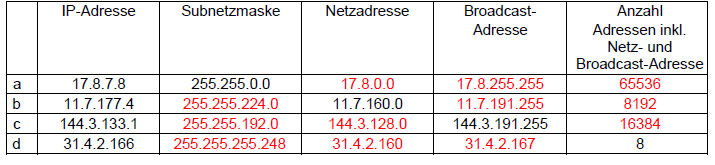
\includegraphics[width=0.8\textwidth]{images/2024-06-20-18-18-53.png}
  \end{center}

\end{example}
\begin{example}{ARP request}\\

  \begin{center}
  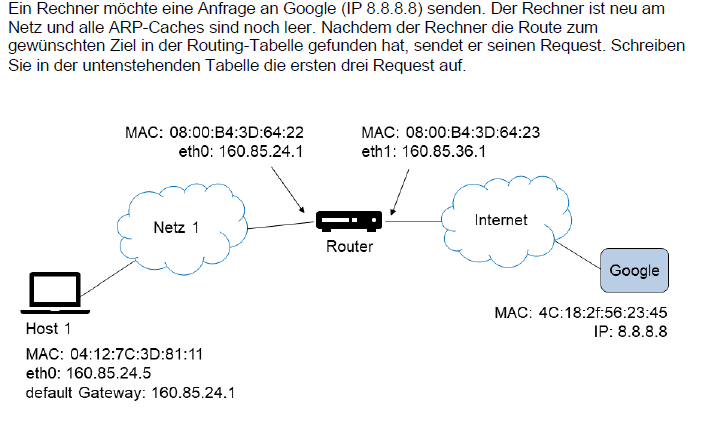
\includegraphics[width=0.8\textwidth]{images/2024-06-20-18-20-15.png}
  \end{center}

  \begin{center}
  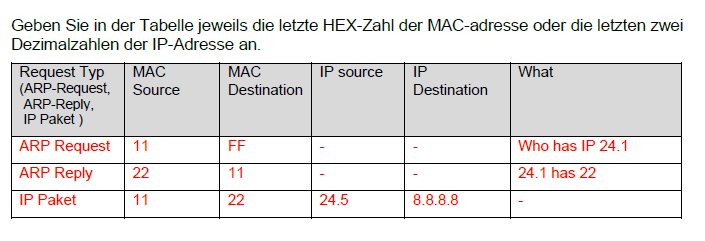
\includegraphics[width=0.8\textwidth]{images/2024-06-20-18-20-33.png}
  \end{center}
\end{example}
